\documentclass[]{article}
\usepackage{graphicx}
\usepackage{hyperref}
\usepackage{listings}
\usepackage{subcaption}
\usepackage{pgfplots}
\usepackage{xcolor}
\usepackage{amsmath}
\usepackage{wrapfig}
\usepackage{makecell}

%opening
\title{IoT-BAsed Indoor Air Quality Monitoring System}
\author{Simone Fabbri}

\lstdefinestyle{C++}{language=C++,
	basicstyle=\ttfamily,
	keywordstyle=\color{blue}\ttfamily,
	stringstyle=\color{red}\ttfamily,
	commentstyle=\color{teal}\ttfamily,
	morecomment=[l][\color{magenta}]{\#}
}


\lstdefinestyle{Python}{language=Python,
	basicstyle=\ttfamily,
	keywordstyle=\color{purple}\ttfamily,
	stringstyle=\color{red}\ttfamily,
	commentstyle=\color{cyan}\ttfamily,
	morecomment=[l][\color{cyan}]{\#}
}


\lstdefinestyle{bash}{
	language=bash,
	basicstyle=\color{orange}\ttfamily,
	keywordstyle=\color{purple}\ttfamily,
	stringstyle=\color{red}\ttfamily,
	commentstyle=\color{violet}\ttfamily
}

\begin{document}

\maketitle

\section{Introduction}
The scope of this project is to make an air quality monitoring system, based on two sensors:
\begin{itemize}
	\item the \texttt{DHT22} sensor, for the temperature and humidity;
	\item the \texttt{MQ-2} sensor, for various gas monitoring (like CO and methane).
\end{itemize}

The sensors are connected to an \texttt{ESP-32} board; the \textit{raw data} is gathered and stored on a InfluxDb instance, and is possible to view it through 2 Grafana dashboards, together with humidity, temperature and gas \textit{predictions}. 

Furthermore, \textbf{2 additional components} are developed:
\begin{itemize}
	\item an \textbf{external temperature} gathering system, which collects the external temperature hourly thanks to the Open API Weather service and the \textbf{meteostat} python library;
	\item a \textbf{telegram bot}, which alerts when the air quality is below a certain threshold and sends a rendered image of the various Grafana panels at regular intervals.
\end{itemize}

The next sessions explain the technical details of how these goals were achieved.

\section{Project's Architecture}
\subsection{Hardware architecture}
The hardware components used in this project are:
\begin{itemize}
	\item \texttt{ESP-WROOM-32}: single board microcontroller, with wifi and bluetooth capabilities; in this project, both available cores and the wifi are used;
	\item \texttt{DHT22}, humidity and temperature sensor;
	\item \texttt{MQ-2}, gas sensor; it can output an analog and a digital signal; the analog signal is used. 
\end{itemize}

While the DHT22 is connected to the 3.3V board output, which is the operating sensor voltage, the MQ-2 is connected to the \texttt{vin} pin, which could also be used as an output voltage pin. A scheme is showed in figure \ref{scheme}.


\begin{figure}[h]
	\centering
	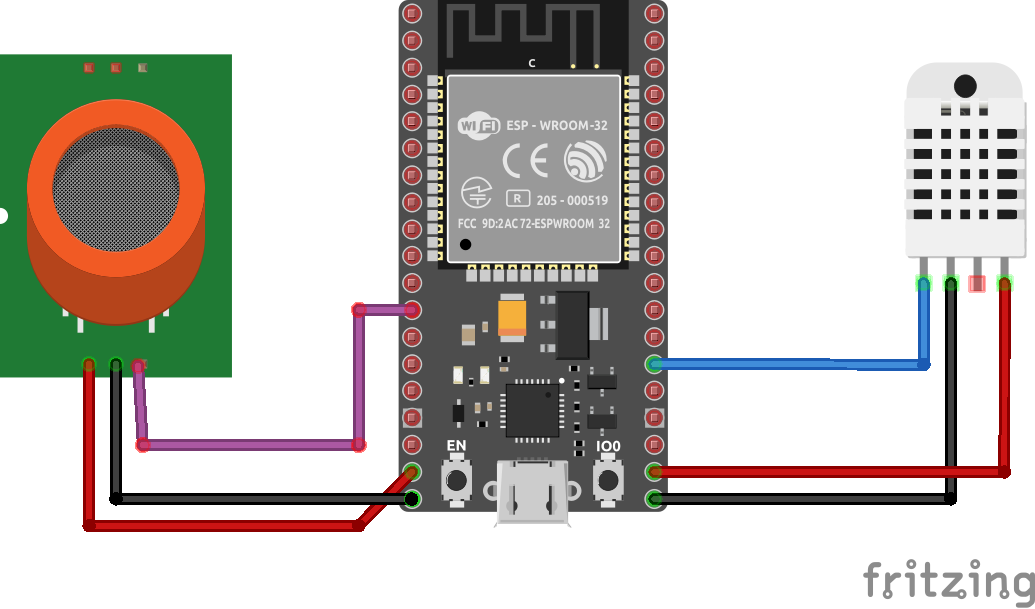
\includegraphics[width=0.6\linewidth]{img/scheme.png}
	\caption{Electric scheme for the project's hardware architecture.}
	\label{scheme}
\end{figure}


\subsection{Software architecture}\label{arch}
The software architecture is composed of the software (and libraries) for the development board, and the software for the various servers and services which run on a computer. 

All the components running in a computer are developed in a docker image: this means that there is an image for the data proxy, an image for the data analytics... All the images where built from scratch, except for Grafana, a plugin called grafana-image-renderer and InfluxDB, which images are already provided from \textit{hub.docker.com}.

All the containers are managed through a \textit{docker compose} file. 

\subsubsection{IoT smart device}
The code for the Esp 32 and the sensors is stored in the \texttt{esp\_32} folder. There are two versions of the code:
\begin{itemize}
	\item \texttt{main}: is the main version of the logic for the board.
	\item \texttt{perf\_eval}: is a simplified version of the main source code, with the only purpose of evaluating the performance (time and packet loss) of the protocols used to exchange sensor data with the data management components. 
\end{itemize}

The (main version of) the IoT smart device logic is in charge of connecting to the network through wifi, acquiring the data and sending it; there are 2 available protocols to do this:
\begin{itemize}
	\item coap;
	\item http.
\end{itemize}

Through the coap protocol is also possible to change some settings, like the interval between the sensor acquisitions, or the \texttt{MIN/MAX\_GAS\_VALUE}. 

To change these settings, an external software is used: \texttt{libcoap2-bin}, available in the linux apt repository. This program provides a binary, \texttt{coap-client}, through which is possible to send messages to a coap server. 

The complete command is \texttt{coap-client -e "TEXT"  -m post coap://URL/set}; this command sends the text \texttt{TEXT} to the \texttt{set} endpoint. The text sent represents the setting we want to change. The possible values are listed in the table \ref{commands} .


\begin{table}
	\centering
	\begin{tabular}{|c|c|c|c|}
		\hline
		\textbf{Command} & \textbf{Parameter} & \textbf{Description} & \textbf{Example} \\
		\hline
		\textit{int} & None & \makecell{Sets the sample \\ frequency, in milliseconds } & \makecell{\texttt{coap-client -e "5000"} \\ \texttt{-m post coap://1.2.3.4/set}} \\
		\hline
		\texttt{c} & None & \makecell{Switch the protocol \\ in which the board \\ sends the data to coap } & \makecell{\texttt{coap-client -e "c"} \\ \texttt{-m post coap://1.2.3.4/set}} \\
		\hline
		\texttt{h} & None & \makecell{Switch the protocol \\ in which the board \\ sends the data to http }  & \makecell{\texttt{coap-client -e "h"} \\ \texttt{-m post coap://1.2.3.4/set}} \\
		\hline
		\texttt{x} & \textit{int} & Sets the gas max value                                         & \makecell{\texttt{coap-client -e "x1000"} \\ \texttt{-m post coap://1.2.3.4/set}} \\
		\texttt{m} & \textit{int} & Sets the gas min value                                         & \makecell{\texttt{coap-client -e "m500"} \\ \texttt{-m post coap://1.2.3.4/set}} \\
		\hline
	\end{tabular} 
	\caption{\label{commands}List of commands understood by the coap server instantiated in the board, through which is possible to change some settings.}
\end{table}

%libcoap2-bin/jammy,now 4.2.1-1build1 amd64
%C-Implementation of CoAP - example binaries API version 2

The code is splitted into several files:
\begin{itemize}
	\item \texttt{main.ino}, contains the two basic functions \texttt{setup()} and \texttt{loop()};
	\item \texttt{settings.h, settings.cpp}: stores some settings like the coap/http server ip addresses and handles the changing of the settings;
	\item \texttt{data.h, data.cpp}: handles getting and sending all the data (sensors, AQI, gps location...).
\end{itemize}

For the performance evaluation, there is also an extra python script in the \texttt{performance\_eval/protocols} folder which is used to analyze the data collected through the \texttt{perf\_eval} version of the logic to control the board. 

\subsubsection{Data proxy}
The data proxy consists in a python module which runs the coap and the http servers.

This server is started from a docker container, which image is defined through a \textbf{Dockerfile}. The ports of these services are exposed to the system. 

Some common settings, like the InfluxDb token, are saved in a common file, \texttt{settings.json}, accessible to all the software components (except of course the ones for the Esp board). The use of this settings file is omitted in the next paragraphs, to avoid repetition.

The coap and http server are based on two libraries, $ aiocoap $  and $ aiohttp $.  

\subsubsection{Data management}
The data management is based on an InfluxDb docker instance and a Grafana docker instance; furthermore, a \textit{Grafana Image Renderer} server is used to render the Grafana panels as images. 

All these components are instantiated through the \textbf{docker compose} file, and the ports are exposed to the system. 

\subsubsection{Data analytics}
The data analytics consist of predicting the values of temperature, humidity and gas from raw values.

This prediction is done by a python module, \texttt{data\_prediction}, which accomplishes this goal thanks to the \textbf{Facebook Prophet library}. 

\subsubsection{Extra components}
There are two extra components, one responsible for getting outdoor meteo information, and the other is the telegram bot. Both components are python modules.

Like the modules above, each run in its separate docker container, defined though its proper Dockerfile, and are instantiated by docker compose. 

\section{Project's Implementation}
\subsection{IoT smart device}
The code for the IoT smart device is divided in several files, briefly introduced in the architecture section \ref{arch}.

The most imporant libraries used to implement the different functions are:
\begin{itemize}
	\item \texttt{coap-simple.h}, for coap communications;
	\item \texttt{WiFi.h}, to connect to a WiFi connection;
	\item \texttt{DHT.h}, to read values from the temperature/humidity sensor;
	\item \texttt{HTTPClient.h}, to send http requests.
\end{itemize}

In the next paragraphs, the relevant content of the various files is described.

The details for the \texttt{perf\_eval} version of this code will be described in the section about the performance evaluation, since the small changes affect only parts specific to the performance evaluation task.
\subsubsection{main}
In this file, the SSID and password for the network to connect is hardcoded in two variables (\texttt{SSID} and \texttt{PASS}). 

In the \texttt{setup()} function, the serial communication, the WiFi connection and the DHT sensor readings are initialized; furthermore, the coap server is also started, to be able to receive commands from a client; this last part is handled by the following instruction:

\begin{lstlisting}[style=C++, caption=Coap server]
// CoAP server endpoint url callback
void coap_change_settings(CoapPacket &packet, IPAddress ip, int port) {
  Serial.println("[Setting something]");
  set(packet);		
  coap.sendResponse(ip, port, packet.messageid, "ok");
}

void setup(){
  //...
  coap.server(coap_change_settings, "set");
}
\end{lstlisting}

The \texttt{set()} function is defined in \texttt{settings.cpp}.

In the \texttt{main} file is also defined the coap callback function (which simply prints the response).

The \texttt{coap.loop()} function is not handled in the main thread, but in another thread, since the ESP 32 has two cores; this means that when we want to change settings, the board can handle the request almost immediately. This is achieved through the system function \texttt{xTaskCreatePinnedToCore()}.

Three things happen in the \texttt{loop()} function: the data is acquired, the data is sent and the thread sleeps for some time, as showed in the listing below:

\begin{lstlisting}[style=C++, caption=Loop function]
void loop() {		
  Serial.println("Getting data...");
  get_data();
  if (TIME_WINDOW[4] >= 0){
    Serial.println("Sending data...");
    send_data();
  }
  delay(SAMPLE_FREQUENCY);	
}
\end{lstlisting}

The functions are defined in \texttt{data.cpp}. Note that the data is not sent immediately, but after 5 times that we collected temperature/humidity/gas; this is because to compute the AQI, we need the mean of 5 measures. In the next section will be described how the array \texttt{TIME\_WINDOW} works.

\subsubsection{data.cpp}
This file has two functions: \texttt{get\_data()} and \texttt{send\_data()}.

The first function reads the temperature and humidity through the \texttt{DHT} library. For the gas, the analog value of the pin where the MQ-2 is connected is read; this value varies between 0 and 4095. \cite{tut:read}

The value of the gas is then inserted in the \texttt{TIME\_WINDOW} array; this array is initially initialized with negative values, so when in \texttt{TIME\_WINDOW[4]} there is a $ \ge 0 $ value, we know we have read at least 5 values, and we can compute the AQI.

When the 6th, 7th, ... and so on read is done, the value is inserted in \texttt{TIME\_WINDOW} in a circular way, starting again from position 0.

All the values are then inserted into a data struct, as the listing below shows:

\begin{lstlisting}[style=C++, caption=Loop function]
struct {
  char temperature[64];
  char humidity[64];
  char AQI[32];
  char gas_conc[32];
  char RSSI[32];
  const char gps[16] = "44.4948,11.3426"; //bologna's coordinates
  const char device_id[18] = "30:C6:F7:22:83:F4"; //mac address
} DATA2SEND;	
\end{lstlisting}

The function \texttt{send\_data()} takes the values from the data structures; in case we want to use coap to transmit them, we first "tag" the data: we append the gps coordinate and the device id to the value we want to send. Then, the data is sent to the appropriate handler.
The example shows the tagged temperature:

\begin{lstlisting}[style=C++, caption=Example of tagged  data (temperature) - coap protocol]
if (PROTOCOL==COAP){
  char tagged_data[50];
  //"tag" the data with gps and device id
  snprintf(tagged_data, 50, "%s;%s;%s", DATA2SEND.temperature, 
    DATA2SEND.gps, DATA2SEND.device_id);
  int msgid = coap.put(IPAddress(COAP_SERVER_IP[0], COAP_SERVER_IP[1], 
    COAP_SERVER_IP[2], COAP_SERVER_IP[3]),
    COAP_PORT, "env/temp", tagged_data);
  //...
}
\end{lstlisting}

If we want to send the data through http protocol, all the data in sent together in json format:

\begin{lstlisting}[style=C++, caption=an http request contains all the data (omitted for simplicity)]
int ret = snprintf(postData, 150, "{\"temp\":%s,\"hum\":%s\" /*...*/ }",
DATA2SEND.temperature, DATA2SEND.humidity /*...*/);
Serial.println("Sending post request...");
http.begin(HTTP_SERVER);
http.POST(postData);
Serial.println("post done");
\end{lstlisting}

\subsubsection{settings.cpp}
This file contains the variables for the coap server ip, the sample frequency for the sensor values... the variables that can be changed are summarized in the table below, with their default values:

\begin{center}
	\begin{tabular}{|c|c|c|}
		\hline
		\textbf{variable} & \textbf{default value} & \textbf{description} \\
		\hline
		\texttt{PROTOCOL} & \texttt{COAP} & protocol in use to send the data \\
		\hline
		\texttt{MIN\_GAS\_VALUE} & 500 & value used for AQI \\
		\hline
		\texttt{MAX\_GAS\_VALUE} & 1500 & value used for AQI \\
		\hline
		\texttt{SAMPLE\_FREQUENCY} & 5000 & sample frequency in ms \\
		\hline
	\end{tabular}
\end{center}

In this file is also defined a function, \texttt{set()}, which sets the variable requested from a client with the new value according to the request. 

\subsection{Data proxy}

The data proxy consist of a python module where are defined the two servers, http and coap, thanks to two libraries: \texttt{aiohttp} and \texttt{aiocoap}.

The servers are run asynchronously as coroutines thanks to the \texttt{asyncio} python library. 

When a request arrives to one of the servers, every server is responsible to create a \texttt{Point} object; this object is defined in the \texttt{influxdb\_client} library. For example, the http server creates this object:

\begin{lstlisting}[style=Python]
d = [
  Point("data")
    .tag("device_id", post_data["id"])
	.tag("location", post_data["gps"])
	.field("rssi", post_data["rssi"]),
  Point("env")
	.tag("device_id", post_data["id"])
	.tag("location", post_data["gps"])
	.field("temperature", post_data["temp"])
	.field("humidity", post_data["hum"])
	.field("aqi", post_data["AQI"])
	.field("gas_concentration", post_data["gas"])]
\end{lstlisting}

then the function \texttt{save\_data()} is called, to save the data to the Influx database. 

Notice how the data is saved in two different \textit{measures}, "data" for the RSSI and "env" for the sensor values and the AQI. 

There is also a function called \texttt{compute\_ppm()}, which takes the raw gas sensor value and computes the ppm of different gases (altough is impossible to know which gas stimulated the sensor in the first place). This computation is performed after some time, because it is necessary to first collect some raw values to compute the \texttt{R0} value (which is the resistance of the sensor in fresh air, without gas - see the appendix \ref{appendix}), which is initially set to 0. When the value becomes different than 0, this function computes the ppms and saves them with the \texttt{save\_data()} function. 

\subsection{Data management}

Data management is performed through an InfluxDB instance, which stores the data and does not require any special configuration, a Grafana instance to visualize the data, and a Grafana image renderer service to render the panels that will later be sent via a telegram bot. 

As regards the Influx instance, some parameters like the token to access the buckets is defined in the \texttt{docker-compose.yml} file, which is used by \texttt{docker compose} to start all the docker services, including Grafana and the image renderer.

In Grafana, there are two dashboards: one for the sensor data, in which is also shown the predictions, the RSSI, the AQI and the data collected from meteostat.

In the second dashboard is shown the ppm for the gases. 

Finally, an alert was defined for the AQI; this is described in section \ref{teleg_sect}. 

\subsection{Data analytics}
The data analytics is composed by another python module, \texttt{data\_predictions}, which is based on the library Prophet by Facebook.

This module predicts $ X $ seconds in the future, according to the \texttt{sample\_frequency} value for the sensors:

\begin{lstlisting}[style=Python, caption=Prophet prediction ($ X $ is \texttt{frequency} in the example)]

future = m.make_future_dataframe(periods = periods, 
	freq=str(frequency) + " S", include_history = False)
forecast = m.predict(future)
\end{lstlisting}

The value of $ X = 100 $ is used in the project. In the code listing, the parameter \texttt{periods} is equal to $ X / \texttt{sample\_frequency} $; \texttt{freq}  is set to the value of \texttt{sample\_frequency}. So, if our sample frequency is 5 seconds (i.e. we have a new value every 5 seconds), this corresponds to a prediction every 5 seconds, for $ X/5 $ times. 

The predictions are then saved in Influx.

The function is executed by the python module periodically, every $ X  $ seconds. The data used to make the predictions is all the raw sensor values from 24 hours before the prediction: so, if $ X = 100 $, if we want to predict the temperature from now, e.g. from 2023-01-01T10:00:00 to 2023-01-01T10:01:40, the module asks to the InfluxDB instance the temperature values from 2022-12-31T10:00:00 to 2023-01-01T10:00:00. 

In case of an exception (likely because there is not enough data to make the first prediction), the module sleeps more before try again. 

\subsection{Extra components}

\subsection{Meteostat}

A python module gets the hourly external temperature of Bologna, using the meteostat library to access the Open API Weather service. 

The system runs every hour, and asks for the temperature of the last hour, and then saves the result in Influx.

\subsection{Telegram bot}\label{teleg_sect}
This is another python module; it is based on the python library \texttt{python-telegram-bot}. 

The bot does not actually interact with the user, but only sends some images and notifies him when the AQI is too low. 

\begin{wrapfigure}{r}{0.5\textwidth}
	\begin{center}
		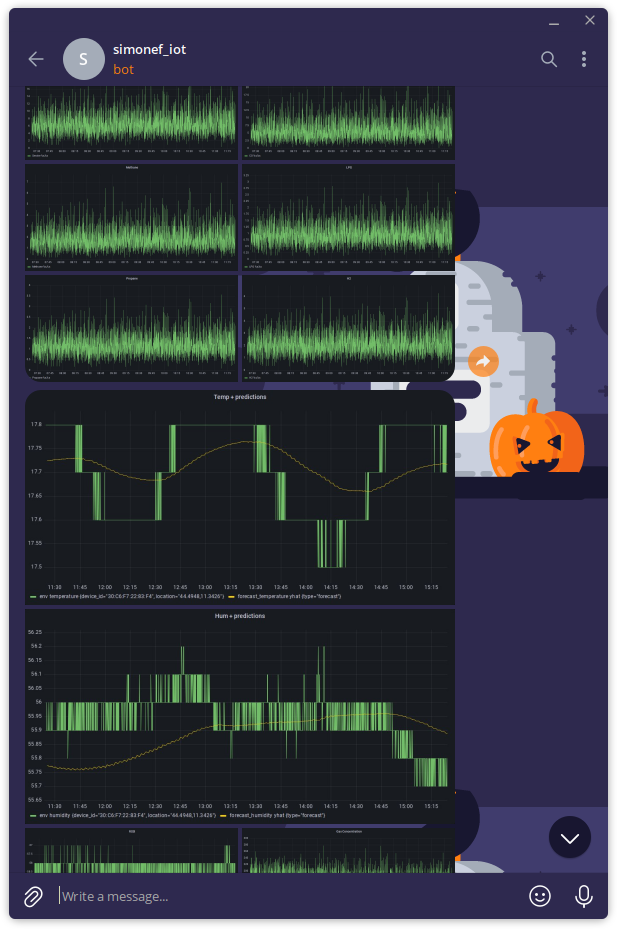
\includegraphics[width=6cm]{img/telegram.png}
		\caption{\label{telegram}Telegram chat with the charts sent by the bot.}
	\end{center}
\end{wrapfigure}

To fulfill the first purpose, first it reads a parameter from the common json settings file, 

\texttt{telegram\_update\_frequency}: this is the frequency of the updates. The bot simply downloads an image of every panel in the Grafana dashboards; the data represented in the charts is from \texttt{telegram\_update\_frequency} hours ago to now. The request is accomplished thanks to the grafana image renderer plugin and the python library \texttt{requests}; after all the images have been collected, they are sent to the user. This is achieved sending a media group to a specific chat id (also read from the json settings).
\\
\\
Regarding the \textbf{AQI alert}, this is a feature of Grafana: a simple contact point was added to use telegram, and configured with the telegram chat id. Then, a rule was added; the rule is composed of three expressions:
\begin{enumerate}
	\item \textbf{Influx query:} a simple query retrieves the AQI values;
	\item \textbf{reduce:} the last element of the query is taken;
	\item \textbf{threshold}: if the element is below 2, the alert is triggered.
\end{enumerate}



\begin{lstlisting}
	
\end{lstlisting}

\section{Results}

In this section the results of various performance tests is discussed. The elements analyzed were:
\begin{itemize}
	\item protocols (http and coap):
	\begin{itemize}
		\item average packet delay
		\item packet delivery ratio
	\end{itemize}
	\item data analytics (Facebook Prophet):
	\begin{itemize}
		\item MSE
	\end{itemize}
\end{itemize}

The results are shown in the following subsections.

\subsection{Protocol evaluation}
For this evaluation, 1000 packets were sent with each protocol, at three different sensor collection frequency values: acquisition every 100ms, 500ms and 1000ms; so in total 6 tests were performed. 

A different version of the main firmware was used: all the serial debugging output messages were deleted (e.g. "board connected to wifi"), and some new were added, as described below.

For the coap protocol, for every packet sent the ESP32 board printed through the serial connection an 'S', the timestamp and the message id; for every packet received, an 'R', the timestamp and the message id. 

The output was collected through the \texttt{screen} command and saved in a csv:

\begin{lstlisting}[style=bash, caption=Command to capture the board serial output]
	screen -L \ 
	   -Logfile perfomance_analysis_coap_500ms.csv \
	   /dev/ttyUSB0 9600
	
	# example of csv file
 	# S, 36984, 256285
	# R, 36984, 256662
	# S, 62982, 256787
	# R, 62982, 257163
\end{lstlisting}

The board did non sent all the sensor data, but just the temperature.

The same approach was used to analyze the http protocol, except in this case was printed the http status code of the request and the total time required to perform it. 

On the server side, the received data was not saved, to avoid the overhead involved in saving the data, since the goal was to analyze the raw protocol performance. 

\subsubsection{Coap}
For the \textbf{coap} protocol, using \texttt{grep S}, \texttt{grep R} and \texttt{wc -l} to count the sent and received packets, we can know how many were lost. This data along some other statistics are shown in the following table:

\begin{table}
\centering
\begin{tabular}{|c|c|c|c|}
	\hline
	\textbf{Measure} & \textbf{100 ms} & \textbf{500 ms} & \textbf{1000 ms} \\
	\hline
	\textit{Packet ratio} & 96.1\% & 95.8\%  & 96.1\% \\
	\hline
	\textit{Average delay} & 278.9 ms & 266.3 ms & 264.6 ms \\
	\hline
	\textit{Min delay} & 7 ms & 7 ms & 6 ms \\
	\hline
	\textit{Max delay} & 575 ms & 596 ms & 788 ms \\
	\hline
	\textit{Median delay} & 278 ms & 273 ms & 261 ms \\
	\hline
\end{tabular} 
\caption{\label{coap}Coap stats table.}
\end{table}

So, in conclusion, increasing the data acquisition (and  thus data sending) frequency did not change the packet loss ratio much, but did positively affect the average and median delay, i.e. decreasing them. 

The delay for every packet is shown in the following images:

\begin{figure}[h]
	\begin{subfigure}{0.5\textwidth}
		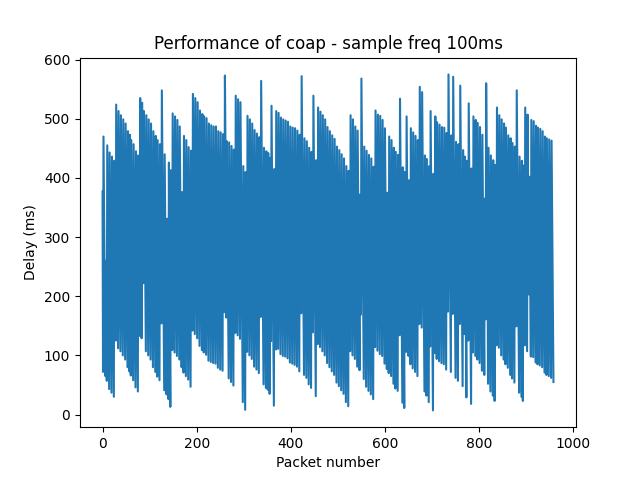
\includegraphics[width=0.9 \linewidth]{../performance_eval/protocols/fig/coap_100ms}
		\caption{}
		\label{fig:coap100ms}
	\end{subfigure}
	\begin{subfigure}{0.5\textwidth}
		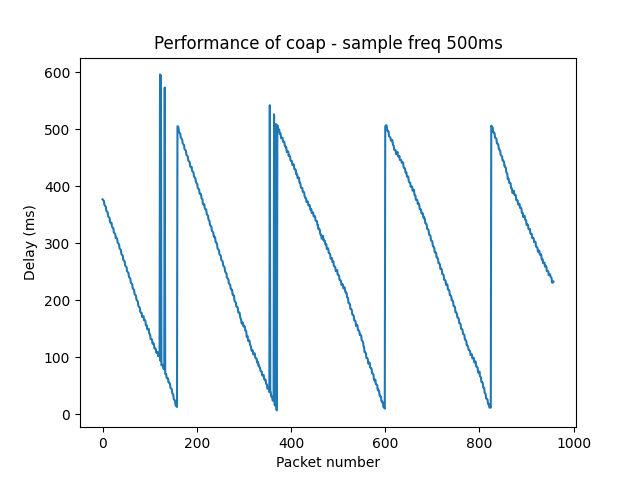
\includegraphics[width=0.9\linewidth]{../performance_eval/protocols/fig/coap_500ms}
		\caption{}
		\label{fig:coap500ms}
	\end{subfigure}	
	\begin{subfigure}{0.5\textwidth}
		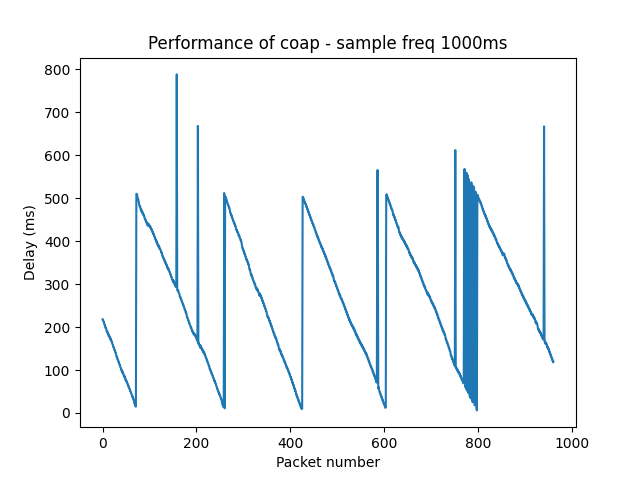
\includegraphics[width=0.9\linewidth]{../performance_eval/protocols/fig/coap_1000ms}
		\caption{}
		\label{fig:coap1000ms}
	\end{subfigure}
	
\end{figure}



As we can see, there is a toothsaw profile, which means that after some fast packets, the delay increased very rapidly, to slowly decrease over time. This phenomenon is exacerbated in the 100 ms test. 

\subsubsection{http}

The same techniques used in the previous section were applied here. In the http protocol, there is no packet loss, since it is based on tcp; in spite of this, some timeout due to the server not responding in time occurred, so the packet ratio is still reported in the table \ref{http} .

\begin{table}
	\centering
	\begin{tabular}{|c|c|c|c|}
		\hline
		\textbf{Measure} & \textbf{100 ms} & \textbf{500 ms} & \textbf{1000 ms} \\
		\hline
		\textit{Packet ratio} & 100\% & 99.7\%  & 99.9\% \\
		\hline
		\textit{Average delay} & 124.6 ms & 251.1 ms & 267.9 ms \\
		\hline
		\textit{Min delay} & 54 ms & 30 ms & 54 ms \\
		\hline
		\textit{Max delay} & 4424 ms & 4515 ms & 4575 ms \\
		\hline
		\textit{Median delay} & 65 ms & 75 ms & 95 ms \\
		\hline
	\end{tabular} 
	\caption{\label{http}Http stats table.}
\end{table}

This shows that, in this setup, while http is more reliable than coap and can be faster on average, the minimum delay is still 9 to 13 times bigger, and also the max delay is 5 to 9 times bigger. 

In the following images the delay packet for every packet is shown:

\begin{figure}[h]
	\begin{subfigure}{0.5\textwidth}
		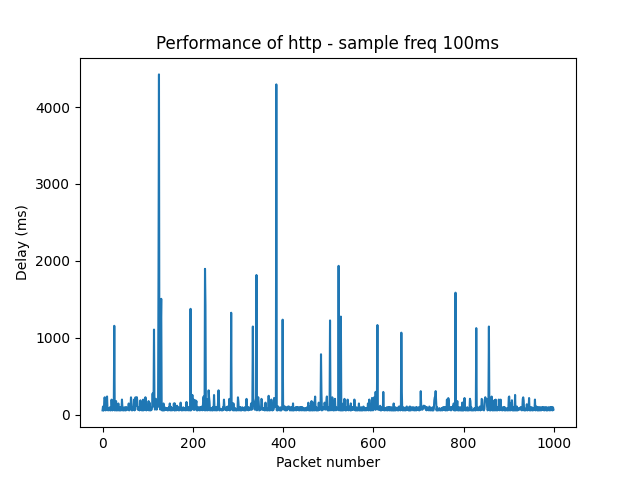
\includegraphics[width=0.9 \linewidth]{../performance_eval/protocols/fig/http_100ms}
		\caption{}
		\label{fig:http100ms}
	\end{subfigure}
	\begin{subfigure}{0.5\textwidth}
		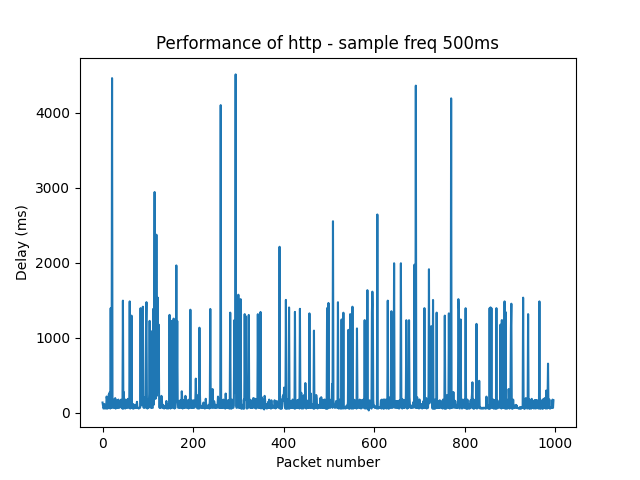
\includegraphics[width=0.9\linewidth]{../performance_eval/protocols/fig/http_500ms}
		\caption{}
		\label{fig:http500ms}
	\end{subfigure}	
	\begin{subfigure}{0.5\textwidth}
		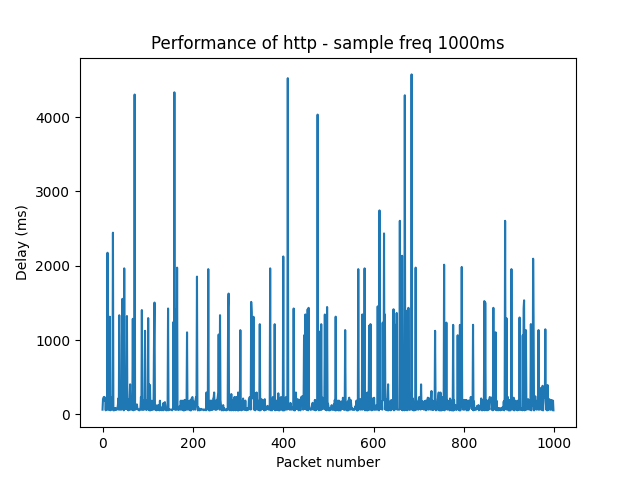
\includegraphics[width=0.9\linewidth]{../performance_eval/protocols/fig/http_1000ms}
		\caption{}
		\label{fig:http1000ms}
	\end{subfigure}
	
\end{figure}

It is possible to observe that the delay is more constant than with the coap protocol, but still peaks of delay are not uncommon. 

\subsection{Data analytics}
In this section Facebook Prophet performance are analyzed. 

Sensor's data was collected for about 2-3 days. Since the goal was to predict the values for X seconds in the future, 100 seconds was chosen as the value for X. Sensor data is collected every 5 seconds, so to match the real data, the predictions were made every 5 seconds. This means every 100 seconds, 20 predictions were made. Before every prediction, the system was fitted with data from the previous 24 hours .

Is it possible to make sub daily predictions with Prophet, as \cite{prophet:subdaily} explains. To better achieve this, we can set a parameter, \texttt{changepoint\_prior\_scale} \cite{prophet:trend_flex}: changepoints are points where the trajectory of the time series changes, and this parameter changes the prior which Prophet uses to estimate the magnitude of the rate change. The bigger this value is, the more flexible we allow the trend to be. The default value is $ 0.05 $.

While collecting sensor's data, a value of $ 0.1 $ was used. After collecting the data, the predictions were made again changing the prior to see if was possible to achieve a lower MSE. The results are shown in the table \ref{rms_table} and the charts \ref{rms_chart}.

The RMS for the $ 0.1 $ prior was computed using data between 2023/01/16, 23:59:59 and 2023/01/17, 23:59:59 (sensor's data and predictions). In order to remake the predictions for the period written above with other priors, the data used to fit Prophet was collected between 2023/01/15, 23:59:59 and 2023/01/17, 23:58:39 (just sensor's data).\footnote{This is because to compute the predictions from, say, 2023/01/17, 01:10:30, to the next 100 seconds (01:11:50) the model used data collected in the previously 24 hours: from 2023/01/16, 01:10:30 to 2023/01/17, 01:10:30.}

\begin{center}
	\begin{table}
		\centering
		\begin{tabular}{|c|c|c|c|}
			\hline
			\textbf{Prior} & \textbf{Rms temperature} & \textbf{Rms humidity} & \textbf{Rms gas concentration} \\
			\hline
			0.001          & 0.0153                 & 1.9485          & 1683.3 \\
			\hline
			\textbf{0.1}   & \textbf{0.0121}        & \textbf{0.3733} & \textbf{1304.5} \\
			\hline
			0.5            & 0.0156                 & 1.9018          & 1709.4 \\
			\hline
			10             & 0.0156                 & 1.9015          & 1713.2 \\
			\hline
		\end{tabular} 
		\caption{\label{rms_table}Rms table for various priors and sensors.}
	\end{table}
\end{center}

\begin{figure}[!h]
	\begin{subfigure}{0.5\textwidth}
		\begin{tikzpicture}
			\node at (2.5,5.2) {Rms for temperature};
			\begin{axis}[width=6cm,height=6cm, xlabel={Prior}, ylabel={rms}]
				\addplot table [x=prior, y=rms, col sep=comma] {../performance_eval/prophet/rms_temperature.csv};
			\end{axis}
		\end{tikzpicture}
	\end{subfigure}
	\begin{subfigure}{0.5\textwidth}
		\begin{tikzpicture}
			\node at (2.5,5.2) {Rms for humidity};
			\begin{axis}[width=6cm,height=6cm, xlabel={Prior}, ylabel={rms}]
				\addplot table [x=prior, y=rms, col sep=comma] {../performance_eval/prophet/rms_humidity.csv};
			\end{axis}
		\end{tikzpicture}
	\end{subfigure}	
	\begin{subfigure}{0.5\textwidth}
	\begin{tikzpicture}
		\node at (2.5,5.2) {Rms for gas concentration};
		\begin{axis}[width=6cm,height=6cm, xlabel={Prior}, ylabel={rms}]
			\addplot table [x=prior, y=rms, col sep=comma] {../performance_eval/prophet/rms_gas_concentration.csv};
		\end{axis}
	\end{tikzpicture}
	\end{subfigure}
	\caption{\label{rms_chart}Rms charts}
\end{figure}

\newpage 

\section*{Appendix}
\appendix
\section{PPM computation}\label{appendix}

The system reads a value from the pin where the gas sensor is connected. Since the sensor is sensible to various gases, it is not possible to know which gas stimulated it. Nevertheless, it is still possible to compute the ppm of the various gas that the sensor can measure \cite{tut:ppm}. 

\begin{figure}[!h]
	\centering
	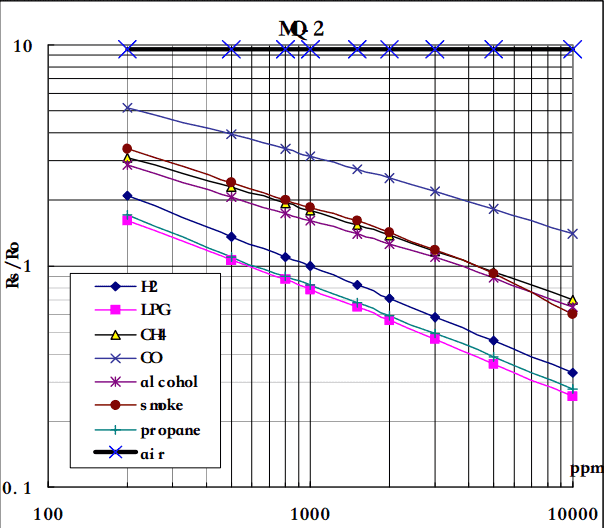
\includegraphics[width=8cm]{img/Gas-Sensor-MQ2.png}
	\caption{\label{mq2table}MQ2 gas sensitivity}
\end{figure}

The input voltage we read from the sensor depends on the amount of gas in the air, and while it depends on the type of gas, can be approximated by the equation of a straight line:

$$ y = mx + b $$

Since the producer of the sensor provides a log scale \ref{mq2table}, the formula becomes:

$$   log(y) = m\cdot log(x) + b   $$

What we want to know is the ppm, which is on the $ x $ axis (and is $ x $ also in the formula); the $ y $ axis, $ RS/R0 $, is the value of the resistance of the sensor in presence of the gas, over the resistance in the fresh air, without concentration of other gases. 

$ RS $ is computed from the input voltage read from the sensor:
$$ RS = (Vin - Vout)/Vout $$

In out case, $ Vin = 3.3 $, and $ Vout = (3.3*analogRead)/4096 $, where \textit{analogRead} is the value we read from the sensor. Since we can read a value between 0 and 4095, \textit{analogRead} is shifted to the 1-4096 range to avoid division by 0. 

Since we know that the resistance ratio in fresh air is a constant: 
$$RS / R0 = 9.8$$
then $ R0 $ is simply:

$$ R0 = RS / 9.8 $$.

To compute $ m $, the slope of the line, it suffices to know two points along the line, and then the formula is:

$$ m = \frac{\log(y_1) - \log(y_0)} {\log(x_1) - \log(x_0)} $$

$ b $ is computed knowing $ m $ and another point in the line:

$$ b = \log(y_3) - m \cdot \log(x_3) $$

Finally, the gas ppm concentration is obtained computing the (inverse log) of x:

\begin{align*}
	log(x) & = 	\frac{\log(y) - b}{m} \\
	x &  = 10 ^ {\frac{\log(y) - b } {m}}
\end{align*}

\begin{thebibliography}{9}
	
	\bibitem{grafana_img} Grafana image renderer plugin, \url{https://grafana.com/grafana/plugins/grafana-image-renderer/}
	
	\bibitem{prophet:subdaily} Sub-daily data, \url{https://facebook.github.io/prophet/docs/non-daily_data.html#sub-daily-data}
	
	\bibitem{prophet:trend_flex} Adjusting trend flexibility, \url{https://facebook.github.io/prophet/docs/trend_changepoints.html#adjusting-trend-flexibility+}
	
	\bibitem{tut:read} ESP32 ADC – Read Analog Values with Arduino IDE,  \url{https://randomnerdtutorials.com/esp32-adc-analog-read-arduino-ide/}
	
	\bibitem{tut:ppm} Interfacing MQ-2 Gas Sensor with evive,  \url{https://thestempedia.com/tutorials/interfacing-mq-2-gas-sensor-with-evive/}
	
\end{thebibliography}

\end{document}

